In order to obtain optimal performance from the neural networks
given a set of atomistic configurations we need a careful choice of parameters
and neural network architecture. The parameters can be classified as either
training parameters - such as learning rate and force loss coefficient -
or architectural parameters - such as the number of neurons and hidden layers,
or the choice of interaction cutoff radius. The former are important
in the training of the neural network, i.e. adjusting weights and biases
while the latter influence both the training process and the final
deployment of the neural networks on unfamiliar data.

\subsection{Force training}
When training the neural networks we have the choice of whether
to incorporate the forces into our loss function, or only fit
the neural network to the potential energy. By default, unless
we have access to a per-atom energy every configuration is labeled
with only a single number for a potentially large number of atoms,
which limits the improvement in loss metrics for every epoch
and the final result. If instead we incorporate the forces into the
loss we have potentially $3N + 1$ labels for every epoch,
which provides a lot more information for weight updates.
In the previous chapter we also showed how adding derivatives to
the loss function could significantly improve the accuracy of the
derivatives. Since the forces determine the trajectories generated
from molecular dynamics we would expect we would expect much better
accuracy and numerical stability if we could improve the fit of
the derivatives.
The real drawback is the calculation of the derivatives in the input layer,
aka the fingerprintprimes, of which there are a lot for every coordinate
and input symmetry function, and they consume a lot of disk space and memory.
\par
In order to test these hypotheses we test the performance of neural networks
trained with and without forces on a set of test images.
A system of copper atoms is generated in the face-centered cubic (FCC)
configuration with 4 atoms in the unit cell and $3 \times 3 \times 3$
unit cells for a total of $4 \cdot 3^3 = 108$ atoms. The
atoms are given velocities from the Maxwell-Boltzmann distribution
corresponding to a temperature of 500 Kelvin. The potential we will
be using is the Effective Medium Theory (EMT), which has a very
fast Fortran implementation in the ASE software package\footnote{
\url{https://wiki.fysik.dtu.dk/asap/asap}}.
The training trajectory is ran for $2 \cdot 10^4$ steps with
a timestep of $\Delta t = 1$fs and written to file every 100 steps
for a total of 200 atomic configurations. The test trajectory is
integrated for $7.5 \cdot 10^3$ steps for a total of 75 atomic configurations.
In table \ref{table:defaults} we have listed the default parameters
used in the training and testing of the neural network:

\begin{table}[h]
\begin{tabular}{@{}lll@{}}
\toprule
\multicolumn{3}{l}{Hyperparameters}                                    \\ \midrule
Architecture & Symmetry functions & AMP defaults (4 radial, 4 angular) \\
             & Hidden layers      & (10, 10)                           \\
             & Activation         & Hyperbolic tangent                 \\
             & Cutoff function    & Polynomial, $R_c = 6.0$            \\
Training     & Epochs             & 2000                               \\
             & Energy coefficient & 1.0                                \\
             & Force coefficient  & 0.1                                \\
             & Optimizer          & BFGS                               \\ \bottomrule
\end{tabular}
\caption{Training defaults}
\label{table:defaults}
\end{table}

\begin{figure}[!tbp]
\begin{adjustbox}{max width=1.2\linewidth,center}
\centering
  \begin{subfigure}[b]{0.55\textwidth}
      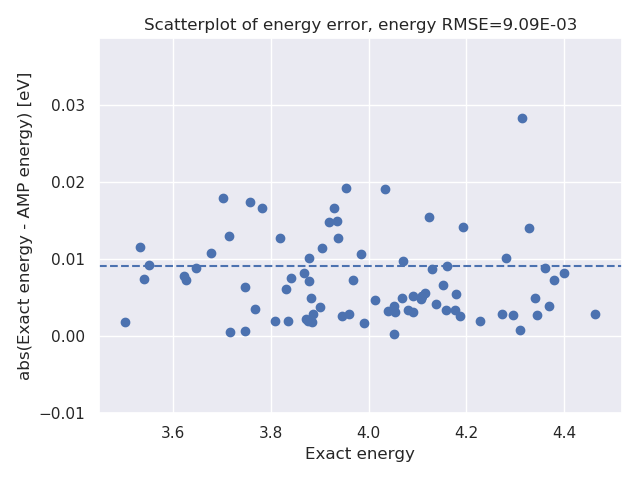
\includegraphics[width=\textwidth]{energy_noforcetrain.png}
    \caption{Flower one.}
    \label{fig:f1}
  \end{subfigure}
  \hfill
  \begin{subfigure}[b]{0.55\textwidth}
      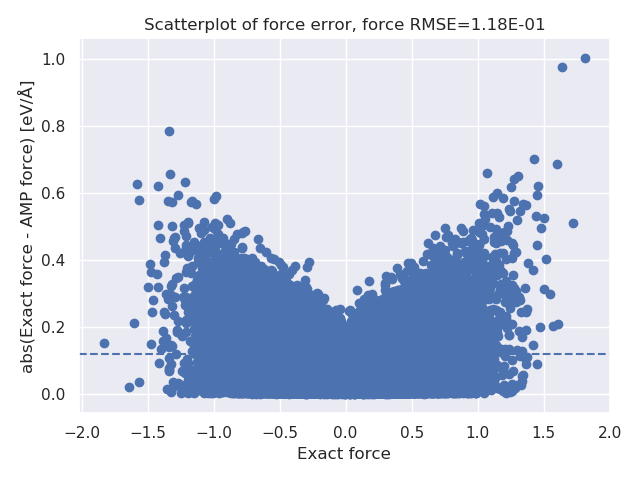
\includegraphics[width=\textwidth]{force_noforcetrain.png}
    \caption{Flower two.}
    \label{fig:f2}
  \end{subfigure}
\end{adjustbox}
\caption{My flowers.}
\end{figure}

\begin{figure}[!tbp]
\begin{adjustbox}{max width=1.2\linewidth,center}
\centering
  \begin{subfigure}[b]{0.55\textwidth}
      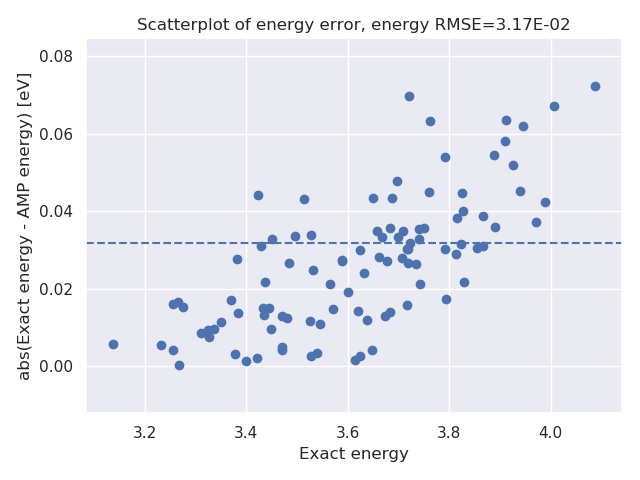
\includegraphics[width=\textwidth]{energy_forcetrain.png}
    \caption{Flower one.}
    \label{fig:f1}
  \end{subfigure}
  \hfill
  \begin{subfigure}[b]{0.55\textwidth}
      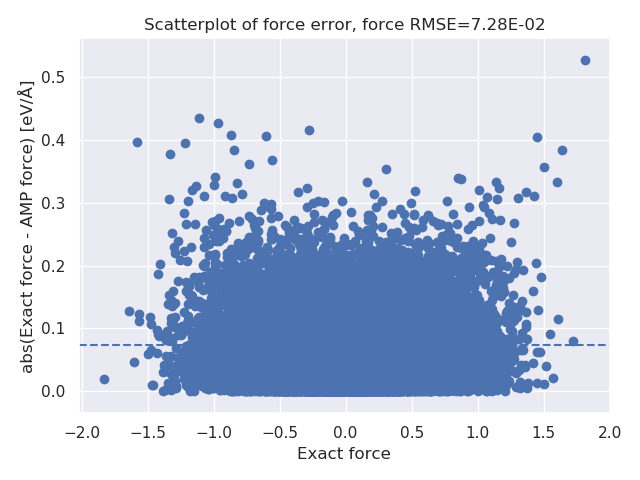
\includegraphics[width=\textwidth]{force_forcetrain.png}
    \caption{Flower two.}
    \label{fig:f2}
  \end{subfigure}
\end{adjustbox}
\caption{My flowers.}
\end{figure}


\subsection{Activation, hidden layers, force coefficient}

\begin{tabular}{lrr}
\toprule
Force coefficient &  Energy RMSE &  Force RMSE \\
\midrule
        0.001 &     4.76E-01 &    4.61E-01 \\
         0.01 &     4.07E-01 &    4.26E-01 \\
          0.1 &     4.54E-01 &    4.07E-01 \\
         0.25 &     3.54E-01 &    4.06E-01 \\
          0.5 &     3.68E-01 &    4.03E-01 \\
\bottomrule
\end{tabular}

\begin{tabular}{llrr}
\toprule
Activation & Hidden layers &  Energy RMSE &  Force RMSE \\
\midrule
      tanh &          10 &     1.84E-01 &    3.43E-01 \\
      tanh &          20 &     1.64E-01 &    3.44E-01 \\
      tanh &          40 &     1.72E-01 &    3.39E-01 \\
      tanh &      10, 10 &     1.73E-01 &    3.37E-01 \\
      tanh &      40, 10 &     1.73E-01 &    3.35E-01 \\
      tanh &      40, 40 &     1.68E-01 &    3.32E-01 \\
   sigmoid &          10 &     1.46E-01 &    3.62E-01 \\
   sigmoid &          20 &     1.75E-01 &    3.45E-01 \\
   sigmoid &          40 &     1.70E-01 &    3.44E-01 \\
   sigmoid &      10, 10 &     1.73E-01 &    3.44E-01 \\
   sigmoid &      40, 10 &     1.80E-01 &    3.42E-01 \\
   sigmoid &      40, 40 &     1.71E-01 &    3.42E-01 \\
\bottomrule
\end{tabular}

\subsection{Cutoff radius}

\begin{tabular}{lrr}
\toprule
         Cutoff &  Energy RMSE &  Force RMSE \\
\midrule
     Cosine-4.0 &     3.60E-02 &    1.41E-01 \\
 Polynomial-4.0 &     3.29E-02 &    1.46E-01 \\
     Cosine-5.0 &     7.46E-02 &    1.72E-01 \\
 Polynomial-5.0 &     8.75E-02 &    2.04E-01 \\
     Cosine-6.0 &     1.41E-01 &    2.68E-01 \\
 Polynomial-6.0 &     2.39E-01 &    4.11E-01 \\
     Cosine-7.0 &     2.37E-01 &    2.86E-01 \\
 Polynomial-7.0 &     4.21E-01 &    3.95E-01 \\
     Cosine-8.0 &     1.82E-01 &    3.31E-01 \\
 Polynomial-8.0 &     1.76E-01 &    4.66E-01 \\
\bottomrule
\end{tabular}

\begin{figure}
    \centering
    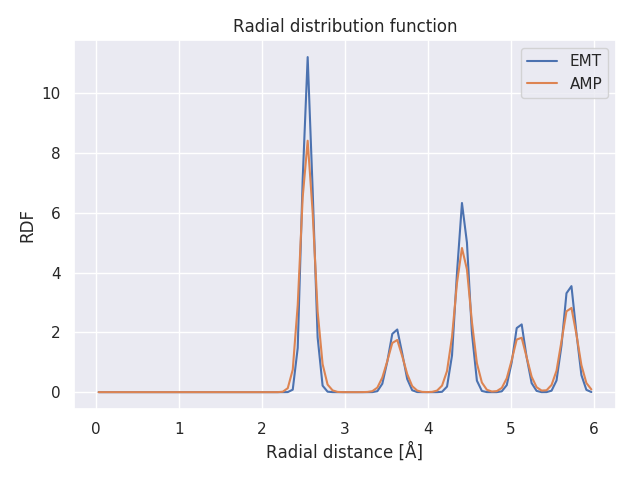
\includegraphics[width=\linewidth]{copper_rdf.png}
    \caption{Copper RDF}
    \label{fig:copper_rdf}
\end{figure}

\subsection{Symmetry functions}

\subsection{Scaling}

